\section{Schedule classification}

Classify the given schedule with respect to CSR (Conflict Serializable) and VSR (View Serializable) classes:
\[r_5(x) r_3(y) w_3(y) r_6(t) r_5(t) w_5(z) w_4(x) r_3(z) w_1(y) r_6(y) w_6(t) w_4(z) w_1(t) w_3(x) w_1(x) r_1(z) w_2(t) w_2(z)\]

\paragraph*{Solution}
To analyze the schedule, we first divide it based on the resources:
\begin{itemize}
    \item $t: \: r_6 \: r_5 \: w_6 \: w_1 \: w_2$
    \item $x: \: r_5 \: w_4 \: w_3 \: w_1$
    \item $y: \: r_3 \: w_3 \: w_1 \: r_6$
    \item $z: \: w_5 \: r_3 \: w_4 \: r_1 \: w_2$
\end{itemize}
The conflict graph is constructed based on write-write or write-read relations in the resource groups. 
The nodes are $\{1,2,3,4,5,6\}$, and the arcs are determined by the conflicts. 
As a result we have the following graph:
\begin{figure}[H]
    \centering
    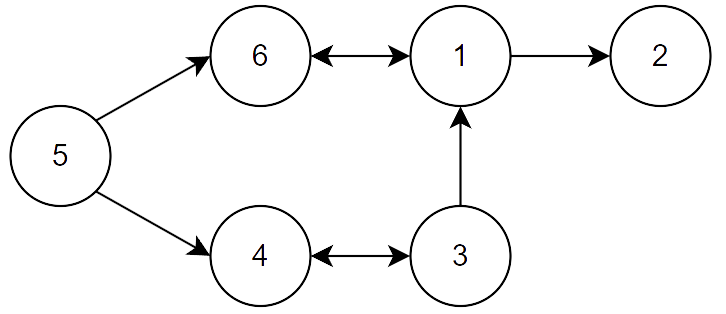
\includegraphics[width=0.5\linewidth]{images/conflictgraph3.png}
\end{figure}

We observe the presence of two cycles in the schedule.
It is unfeasible to discover a VSR (View Serializable) schedule since only the conflict between transactions four and three can be resolved; attempting to address the other cycle would necessitate altering a read-write relation.